% Second section

\section{Literature review: Dynamic scheduling techniques}

Rolling horizon approaches are common strategies in the literature to solve the dynamic scheduling problems. They generally consist in subdividing the planing horizon into smaller sub-horizons. Then solve the (static) problem on each sub-horizon sequentially, as illustrated in Figure~\ref{fig:rh}.
These approaches represent valid solution methods to tackle the dynamic case, because their computation times are usually suitable for real-time applications.

\begin{figure}[h!]
	\centering
	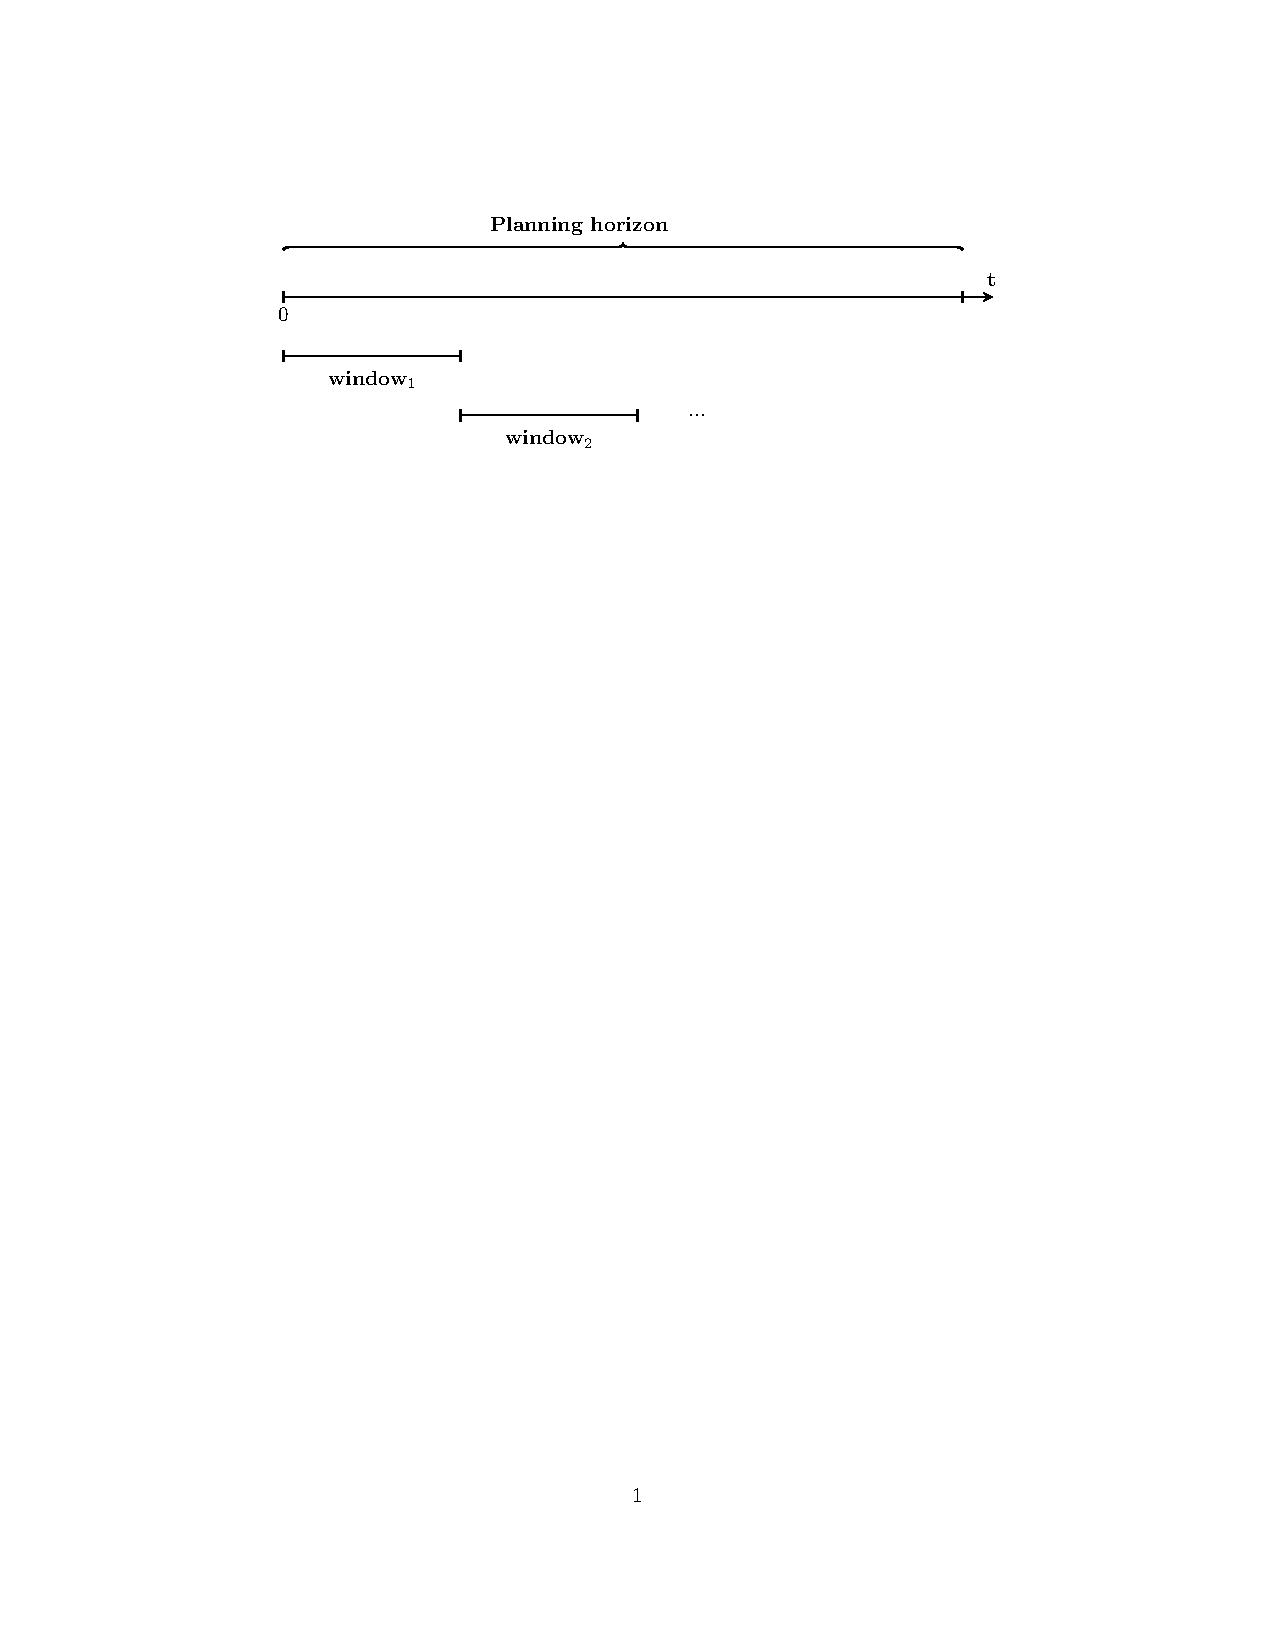
\includegraphics[trim=120 575 120 100,clip,width=0.85\textwidth]{images/rh.pdf}
	\caption{Illustration of the rolling-horizon approach.}
	\label{fig:rh}
\end{figure}
In the next subsection we review the most relevant \acs{RH} approaches for three optimization problems: the job-shop scheduling, the vehicle routing problem, and the unmanned ariel vehicle scheduling problem.


\subsection{Job-Shop Scheduling}
\label{subsec:machine}

In the \acs{RH} approaches for the Job-Shop Scheduling Problem (\acs{JSSP}), there are jobs that will start inside a sub-horizon and finish outside that horizon, regardless of its length. This kind of jobs is called \textit{cross-window} jobs. To deal with them, boundary conditions have to be defined for each sub-horizon. On the other hand, the computation complexity is expected to be reduced in the sub-horizons, since the problem size is smaller. The \acs{RH} scheduling approaches can be categorized into two types of strategies:

\begin{itemize}
	\item The \textit{event-driven} scheduling in which the rolling horizon is a job window, \textit{i.e.}, a number of jobs for scheduling and processing. This strategy first chooses a job window, which is defined by the (allowed) maximum number of jobs. Then, it divides the set of jobs in three sub-sets:
	\begin{enumerate*}[label=(\roman*)]
		\item the sub-set of available jobs,
		\item the sub-set of current jobs, and
		\item the sub-set of finished jobs.
	\end{enumerate*}
	
	A selection rule is then used to select jobs from the sub-set of available jobs. Finally, an optimization algorithm is required to solve the problem in the job windows, and the three above-mentioned sets are updated until all the jobs are processed. Notable examples from the literature that use this approach are~\cite{chen2017,fang1997}. The former work used this strategy to solve the online workflow scheduling on cloud environment, and the latter used it for the classical dynamic \acs{JSSP}.
	
	
	\item The \textit{periodic scheduling} strategies in which the rolling domain is a \textit{time window}, \textit{i.e.}, a time slot on the scheduling horizon. This strategy is used in~\cite{sun1994} to solve the dynamic JSSP. In this work, the authors subdivide the planning horizon, $T$, into two non-overlapping windows, $T_{1}$ and $T_{2}$. Then, they solve the (static) problem on $T_{2}$. Finally, they determine the set of cross-window jobs and schedules them with the jobs in the window $T_{1}$.  
	
	The periodic scheduling is also used in~\cite{tang2010}, but with a different \textit{rolling time-window}. In this context, the planning horizon, denoted $[0,K]$, is subdivided in $R$ time periods of equal lengths. Then, the problem is solved in the whole planing horizon at the beginning. As time progresses, the window is shortened by one time period, and the problem is again solved in the new window, as illustrated in Fig.~\ref{fig:tw-whole}.
	
	
	\begin{figure}[h!]
		\centering
		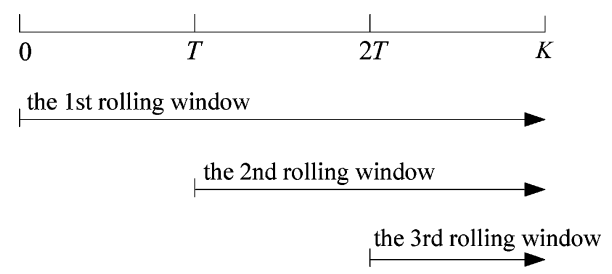
\includegraphics[width=.6\textwidth]{images/tw-whole}
		\caption{A rolling horizon with three time-windows (source:~\cite{tang2010}).}
		\label{fig:tw-whole}
	\end{figure}
	
\end{itemize}



\subsection{Vehicle Routing Problem}

In the dynamic \acs{VRP}, the customer orders are usually considered to be the dynamic events. In the work of Hanshar and Ombuki-Berman~\cite{hanshar2007}, the \acs{RH} periodic scheduling strategy is used, but with time-windows that differs from~\cite{sun1994} and~\cite{tang2010}. Indeed, in~\cite{hanshar2007} , the authors subdivide the planing horizons into several slices of equal lengths. Then, they sequentially solve the (static) VRP on each slice. Furthermore, the authors define a cutoff time, which postpones the late orders to the next day. The genetic algorithm is then used to solve the static problem on each time slice.

A number of heuristics are proposed in~\cite{larsen2002} to solve the dynamic VRP:

\begin{itemize}
	\item First-Come First-Served (FCFS) that serves the clients in the order which they are. A special case of this strategy is:
	
	\item Stochastic Queue Median (SQM) in which the vehicle travels directly from the median of the service region to the next demand location. After the service has been completed, the server returns to the median and waits for the next demand.
	
	\item Nearest Neighbor (NN) that completes the demands in one location, and then travels to the nearest neighboring demand.
\end{itemize}




\subsection{Unnamed Ariel Vehicle Scheduling}

The works in the literature addressing the real-time scheduling and routing of air taxis are rare compared to the machine scheduling or the VRP. Nonetheless, the two recent works~\cite{rajendran2021} and \cite{song2016} consider this dynamic scheduling for two types of air vehicles: the flying taxis for the former work, and the Unmanned Aerial Vehicle (\acs{UAV}) for the latter.

In\cite{song2016}, the authors develop a real-time tool to manage a fleet of \acs{UAV}s to serve customers. The management includes visiting the service station for battery recharging. The problem is formulated as a mixed-integer program, inspired from the \acs{VRP} literature, and solved using \textit{CPLEX}~\cite{cplex2009v12}. The dynamic scheduling is tackled using the \textit{event-driven} and the \textit{periodic scheduling} strategies explained in section~\ref{subsec:machine}.


In the very recent work of~\cite{rajendran2021}, the author considers the real-time dispatching of air taxis in a centralized taxi network. Two objectives are taken into account in the optimization model: minimizing  the \textbf{number of idle taxis} and minimizing the \textbf{total travel time of air taxis at inactive state}. Since these two objectives are conflicting, the author uses a \textit{goal programming} algorithm to solve the problem. The proposed strategy to handle the real-time demands is similar to the one used in~\cite{sun1994}. To the best of our knowledge, this is the only work in the literature that considers the dynamic scheduling of flying taxi.


























